\documentclass[11pt]{article}
\usepackage[utf8]{inputenc}
\usepackage[margin=1in]{geometry}
\usepackage{amsmath,amssymb}
\usepackage{graphicx}
\usepackage{booktabs}
\usepackage{float}
\usepackage[font=small]{caption}
\usepackage[numbers,sort&compress]{natbib}
\usepackage{microtype}
\usepackage[hidelinks]{hyperref}
\usepackage{url}

% generated by code/11_arxiv.py; do not edit
\newcommand{\AuthorName}{Selorm Buaka}
\newcommand{\AuthorAff}{University of Northern Colorado}
\newcommand{\AuthorEmail}{othnielbuaka@gmail.com}
\newcommand{\AuthorOrcid}{0009-0005-3991-4859}
\newcommand{\TrainYears}{2016, 2017 and 2023 (80\% of records)}
\newcommand{\TuneYear}{2023 (held-out 20\%)}
\newcommand{\TestYear}{2024}
\newcommand{\YearsAll}{2016, 2017, 2023, 2024}
\newcommand{\NCohortTotal}{14,509,548}
\newcommand{\NCohortTest}{3,510,372}
\newcommand{\NTeacher}{3,000,000}
\newcommand{\NStudentTrain}{1,000,000}
\newcommand{\NStates}{51}
\newcommand{\NStateStudents}{8}
\newcommand{\NTopStates}{6}
\newcommand{\StudentStates}{Alaska, California, District of Columbia, Hawaii, Montana, North Dakota, Oregon, Washington}
\newcommand{\EvalN}{200,000}
\newcommand{\NaturalN}{200,000}
\newcommand{\Kfold}{5}
\newcommand{\KDalpha}{0.3}
\newcommand{\KDtau}{1.0}
\newcommand{\BootB}{200}
\newcommand{\AlertPct}{10\%}
\newcommand{\SensTarget}{80\%}
\newcommand{\LGBMlr}{0.05}
\newcommand{\LGBMleaves}{63}
\newcommand{\LGBMminleaf}{500}
\newcommand{\LGBMstop}{50}
\newcommand{\MARbeta}{1}
\newcommand{\MARrho}{0.5}
\newcommand{\WTeen}{1}
\newcommand{\WUnmarried}{1}
\newcommand{\WForeignBorn}{0.5}
\newcommand{\WNhWhite}{$-$0.5}
\newcommand{\WHighParity}{0.5}
\newcommand{\StressMult}{5}
\newcommand{\RateMin}{0.1\%}
\newcommand{\RateMax}{4.8\%}
\newcommand{\PrevLBW}{6.9\%}
\newcommand{\TeacherLBWTrees}{378}
\newcommand{\LBWKDsAuc}{0.683}
\newcommand{\LBWKDsPpv}{18.1}
\newcommand{\LBWKDsPpvGap}{+0.10}
\newcommand{\LBWKDpAuc}{0.683}
\newcommand{\LBWKDpPpv}{18.2}
\newcommand{\LBWKDpPpvGap}{+0.11}
\newcommand{\LBWBthreesAuc}{0.682}
\newcommand{\LBWBthreesPpv}{18.1}
\newcommand{\LBWBthreesPpvGap}{+0.01}
\newcommand{\LBWBoneAuc}{0.683}
\newcommand{\LBWBonePpv}{18.0}
\newcommand{\LBWBonePpvGap}{$-$0.03}
\newcommand{\LBWBtwoAuc}{0.682}
\newcommand{\LBWBtwoPpv}{17.9}
\newcommand{\LBWBtwoPpvGap}{$-$0.09}
\newcommand{\LBWBfourAuc}{0.655}
\newcommand{\LBWBfourPpv}{16.6}
\newcommand{\LBWBfourPpvGap}{$-$1.44}
\newcommand{\LBWTAuc}{0.684}
\newcommand{\LBWTPpv}{18.0}
\newcommand{\LBWKDhigherAuc}{8}
\newcommand{\LBWKDhigherPpv}{7}
\newcommand{\LBWKDlowerIci}{1}
\newcommand{\LBWNatEvents}{18,772}
\newcommand{\LBWNatKDAuc}{0.683}
\newcommand{\LBWNatKDPpv}{24.6}
\newcommand{\LBWNatAucOne}{+0.004 to +0.006}
\newcommand{\LBWNatPpvOne}{+0.01 to +0.61}
\newcommand{\LBWNatAucTwo}{+0.013 to +0.016}
\newcommand{\LBWNatPpvTwo}{+0.97 to +1.61}
\newcommand{\LBWNatAucThree}{+0.001 to +0.003}
\newcommand{\LBWNatPpvThree}{$-$0.05 to +0.39}
\newcommand{\LBWNatAucFour}{+0.031 to +0.036}
\newcommand{\LBWNatPpvFour}{+1.95 to +2.77}
\newcommand{\PrevPTB}{8.5\%}
\newcommand{\TeacherPTBTrees}{286}
\newcommand{\PTBKDsAuc}{0.671}
\newcommand{\PTBKDsPpv}{22.7}
\newcommand{\PTBKDsPpvGap}{$-$0.15}
\newcommand{\PTBKDpAuc}{0.671}
\newcommand{\PTBKDpPpv}{22.7}
\newcommand{\PTBKDpPpvGap}{$-$0.10}
\newcommand{\PTBBthreesAuc}{0.669}
\newcommand{\PTBBthreesPpv}{22.7}
\newcommand{\PTBBthreesPpvGap}{$-$0.19}
\newcommand{\PTBBoneAuc}{0.671}
\newcommand{\PTBBonePpv}{22.8}
\newcommand{\PTBBonePpvGap}{$-$0.05}
\newcommand{\PTBBtwoAuc}{0.670}
\newcommand{\PTBBtwoPpv}{22.7}
\newcommand{\PTBBtwoPpvGap}{$-$0.11}
\newcommand{\PTBBfourAuc}{0.644}
\newcommand{\PTBBfourPpv}{21.4}
\newcommand{\PTBBfourPpvGap}{$-$1.44}
\newcommand{\PTBTAuc}{0.672}
\newcommand{\PTBTPpv}{22.8}
\newcommand{\PTBKDhigherAuc}{8}
\newcommand{\PTBKDhigherPpv}{7}
\newcommand{\PTBKDlowerIci}{0}
\newcommand{\PTBNatEvents}{23,492}
\newcommand{\PTBNatKDAuc}{0.685}
\newcommand{\PTBNatKDPpv}{31.6}
\newcommand{\PTBNatAucOne}{+0.009 to +0.011}
\newcommand{\PTBNatPpvOne}{+0.24 to +0.63}
\newcommand{\PTBNatAucTwo}{+0.016 to +0.018}
\newcommand{\PTBNatPpvTwo}{+0.75 to +1.25}
\newcommand{\PTBNatAucThree}{+0.002 to +0.004}
\newcommand{\PTBNatPpvThree}{+0.05 to +0.43}
\newcommand{\PTBNatAucFour}{+0.036 to +0.041}
\newcommand{\PTBNatPpvFour}{+1.94 to +2.82}
\newcommand{\NStudentsCompared}{8}
\newcommand{\SubCells}{30}
\newcommand{\SubTight}{22}
\newcommand{\SubBfourLow}{22}


\title{Missingness-Aware Knowledge Distillation for Low Birthweight and Preterm Birth Prediction under State-Specific Item Missingness in U.S.\ Birth Certificates}
\author{\AuthorName\\ \AuthorAff\\ \small ORCID \AuthorOrcid\\ \small \href{mailto:\AuthorEmail}{\AuthorEmail}}
\date{\today}

\begin{document}
\maketitle

\begin{abstract}
Birth-certificate items that carry much of the antenatal signal for perinatal risk prediction (month prenatal care began, pre-pregnancy body mass index, WIC participation, smoking before pregnancy, maternal education and payer) are also the items most often left unknown, and their completeness differs across U.S.\ states. Models developed on complete records are therefore deployed under missingness they never saw. We evaluate missingness-aware knowledge distillation (MAKD): a gradient-boosted teacher is trained on records complete for all six items, and students are distilled from its cross-fitted soft predictions to operate under each state's observed missingness. Using NCHS public-use natality files (\YearsAll) and state item-completeness rates from CDC WONDER, we imposed the missingness of \NStates{} jurisdictions on national records under completely-at-random and covariate-dependent mechanisms and compared students with imputation, missing-indicator and non-distilled baselines on sensitivity and positive predictive value (PPV) at a \AlertPct{} alert rate, calibration, and subgroup performance in \TestYear{} births. Test-year prevalence was \PrevLBW{} for low birthweight (LBW) and \PrevPTB{} for preterm birth (PTB). At the missingness rates states actually report, all tree-based methods stayed within a fraction of a percentage point of the full-information teacher's PPV, and the best method differed by outcome. On \NaturalN{} real \TestYear{} records with naturally missing items, the pooled distilled student had the highest discrimination for both outcomes, with paired bootstrap intervals for its AUROC advantage over mean imputation (LBW \LBWNatAucOne; PTB \PTBNatAucOne) and iterative imputation (LBW \LBWNatAucTwo; PTB \PTBNatAucTwo) excluding zero. Evaluating models on naturally incomplete records, not only on simulated masks, changed the conclusion about which missing-data strategy to prefer.
\end{abstract}

\noindent\textbf{Keywords:} knowledge distillation, missing data, clinical prediction models, low birthweight, preterm birth, birth certificates, vital statistics.

\section{Introduction}

Low birthweight and preterm birth remain leading contributors to neonatal morbidity and mortality in the United States, and risk models built on birth-certificate data are attractive because those data cover every registered birth. The variables that carry much of the antenatal signal, however, are also the items most often left unknown on the certificate, and completeness for each item differs from one state to another. A model developed on records where these items are complete will be deployed in jurisdictions where they are not, and the size of that gap depends on where the model is used.

Knowledge distillation offers a way to carry what a full-information model has learned into a model that must work with less. A teacher model trained with full information produces soft predictions, and a student model learns to reproduce them from a reduced set of inputs \citep{hinton2015}. U.S.\ vital records suit this design: millions of records are complete on every item and can train a teacher, while each state's actual pattern of unknown items defines the conditions its student must work under.

In this work we evaluate missingness-aware knowledge distillation (MAKD) for predicting low birthweight and preterm birth from antenatal birth-certificate items. Because the public-use natality files carry no state identifier, we impose each state's observed item-unknown rates from CDC WONDER on national records and compare distilled students with imputation, missing-indicator and non-distilled baselines on the measures that matter when an outcome is rare: sensitivity and positive predictive value at a fixed alert rate, calibration, and subgroup performance. We also evaluate every model on real records whose items are naturally missing, the one test that does not depend on a simulated missingness mechanism. This work extends the author's earlier neonatal outcome prediction study in Ghana (manuscript under review) to U.S.\ national data.

The remainder of this article is organized as follows. Section~\ref{sec:related} reviews related work on missing predictors at deployment and on distillation. Section~\ref{sec:methods} describes the data, missingness masks, models and evaluation. Section~\ref{sec:results} reports results, Section~\ref{sec:discussion} discusses them, and Section~\ref{sec:conclusion} concludes.

\section{Related work}\label{sec:related}

The prediction literature has examined how to handle predictors that are missing when a model is applied. Hoogland and colleagues compared strategies for validating and applying a prediction model to patients with missing predictor values \citep{hoogland2020}. Sperrin and colleagues argued that missing data should be handled differently for prediction than for description or causal explanation, favoring approaches that are available at the moment of prediction \citep{sperrin2020}. Sisk and colleagues showed in simulation that imputation and missing-indicator strategies perform differently depending on whether missingness is informative \citep{sisk2023}. These approaches either train each model on the information it will see or fill in what is missing before applying a model trained on complete data. A separate line of work treats a change in missingness between training and deployment sites as a form of distribution shift and adapts the model to the new site \citep{zhou2023}.

Knowledge distillation was introduced to compress a large model into a smaller one by training the smaller model on the larger model's softened outputs \citep{hinton2015}. When the teacher has access to information the student will never see, the arrangement is known as learning with privileged information, and distillation provides a principled way to transfer what the privileged features teach \citep{lopezpaz2016}. Treating the items that are often unknown on a birth certificate as privileged information connects these two literatures: the teacher sees every item, and each student sees only what a given state's records are likely to contain.

\section{Materials and Methods}\label{sec:methods}

\subsection{Data}

We used live births in the NCHS natality public-use files \citep{nchs2024files} for \YearsAll. The cohort was restricted to singleton births to U.S.-resident mothers with stated birthweight and an obstetric-estimate gestational age between 20 and 44 weeks, giving \NCohortTotal{} births across the four years (\NCohortTest{} in \TestYear). Training years were \TrainYears; the tuning year was \TuneYear; the test year was \TestYear. Parsed record counts for U.S.\ residents matched the registered-birth totals in the National Vital Statistics Reports exactly \citep{osterman2026}.

Public-use files carry no state identifier, so state-specific missingness was taken from CDC WONDER Natality (Expanded) \citep{wonder2026}: for each state and item, the proportion of \TestYear{} births with the item unknown or not stated. The national unknown rate for each item in WONDER agreed with the microdata to within 0.01 percentage points.

\subsection{Outcomes and predictors}

Low birthweight (LBW) was defined as birthweight below 2{,}500\,g and preterm birth (PTB) as obstetric-estimate gestation below 37 completed weeks. Predictors were restricted to information available before labor: maternal age, race and Hispanic origin, nativity, marital status, whether the father's age was reported, live-birth order, prior live births and prior other pregnancy outcomes, pre-pregnancy diabetes and hypertension, previous preterm birth, infertility treatment, number of previous cesareans and birth year, plus the six items subject to missingness (month prenatal care began, pre-pregnancy BMI, WIC participation, cigarettes per day before pregnancy, maternal education and payer). Prenatal visit count, delivery and infant items were excluded to avoid leakage.

\subsection{Missingness masks}

For record $i$, item $j$ and state $s$, the probability that the item is masked is
\begin{equation}
P(M_{ij}=1 \mid z_i) = \operatorname{expit}(c_{sj} + \beta z_i),
\end{equation}
where $z_i$ is a standardized weighted score of always-observed covariates (maternal age under 20, weight \WTeen; unmarried, \WUnmarried; foreign-born, \WForeignBorn; non-Hispanic White, \WNhWhite; live-birth order four or higher, \WHighParity) and $c_{sj}$ is solved numerically so that the mean probability equals the state's WONDER rate. Setting $\beta=0$ with independent items gives a missing-completely-at-random (MCAR) mechanism. The missing-at-random (MAR) mechanism used $\beta=\MARbeta$ with within-record dependence between items from a one-factor Gaussian copula ($\rho=\MARrho$), which preserves each item's marginal probability. A stress arm multiplied every state's observed rates by \StressMult, capped at 95\%, to show behavior under much poorer completeness than any state reports.

\subsection{Teacher, students and baselines}

The teacher was a gradient-boosted tree model (LightGBM \citep{ke2017}; learning rate \LGBMlr, \LGBMleaves{} leaves, at least \LGBMminleaf{} records per leaf, early stopping after \LGBMstop{} rounds on the tuning year) trained on \NTeacher{} training records complete for all items. Its soft targets were produced by \Kfold-fold cross-fitting, so that each training record's target came from a model that had not seen it. Each student used the same learner on masked inputs plus missingness indicators and \NStudentTrain{} training records, and was trained with cross-entropy against
\begin{equation}
q_i = \alpha\, y_i + (1-\alpha)\, \operatorname{expit}\!\big(\operatorname{logit}(p^{T}_i)/\tau\big),
\end{equation}
with $\alpha=\KDalpha$ and $\tau=\KDtau$, where $p^T_i$ is the teacher's out-of-fold prediction. Per-state students were trained for \NStateStudents{} states (the \NTopStates{} with the highest mean unknown rate, the median state and the lowest: \StudentStates), and one pooled student was trained over the births-weighted mixture of all \NStates{} jurisdictions' masks.

Baselines were the teacher with mean or mode imputation (B1); the teacher with chained-equation imputation \citep{pedregosa2011} (B2); the student's learner trained on hard labels only (B3, the distillation ablation); and logistic regression with missing indicators (B4).

\subsection{Evaluation}

Each model was evaluated in \EvalN{} test-year births under each state's mask. Thresholds for the \AlertPct{} alert rate and for \SensTarget{} sensitivity were fixed in the tuning year under the same mask and then applied to the test year. Measures were the area under the ROC curve (AUROC), the area under the precision--recall curve (AUPRC), sensitivity and PPV at both operating points, calibration intercept and slope, the integrated calibration index (ICI) \citep{austin2019}, and the Brier score. Uncertainty was quantified by a stratified bootstrap (\BootB{} replicates) for the lowest-, median- and highest-missingness states and for paired differences between models. Subgroups were maternal race and Hispanic origin, age band, payer and nativity. A separate analysis used a random sample of \NaturalN{} test-year records with at least one naturally missing item, with models trained under MAR masks.

\section{Experiments and Results}\label{sec:results}

Test-year prevalence was \PrevLBW{} for LBW and \PrevPTB{} for PTB. Observed state missingness was low: across \NStates{} jurisdictions the mean unknown rate over the six items ranged from \RateMin{} to \RateMax{} (Figure~\ref{fig:missing}).

\begin{figure}[H]
\centering
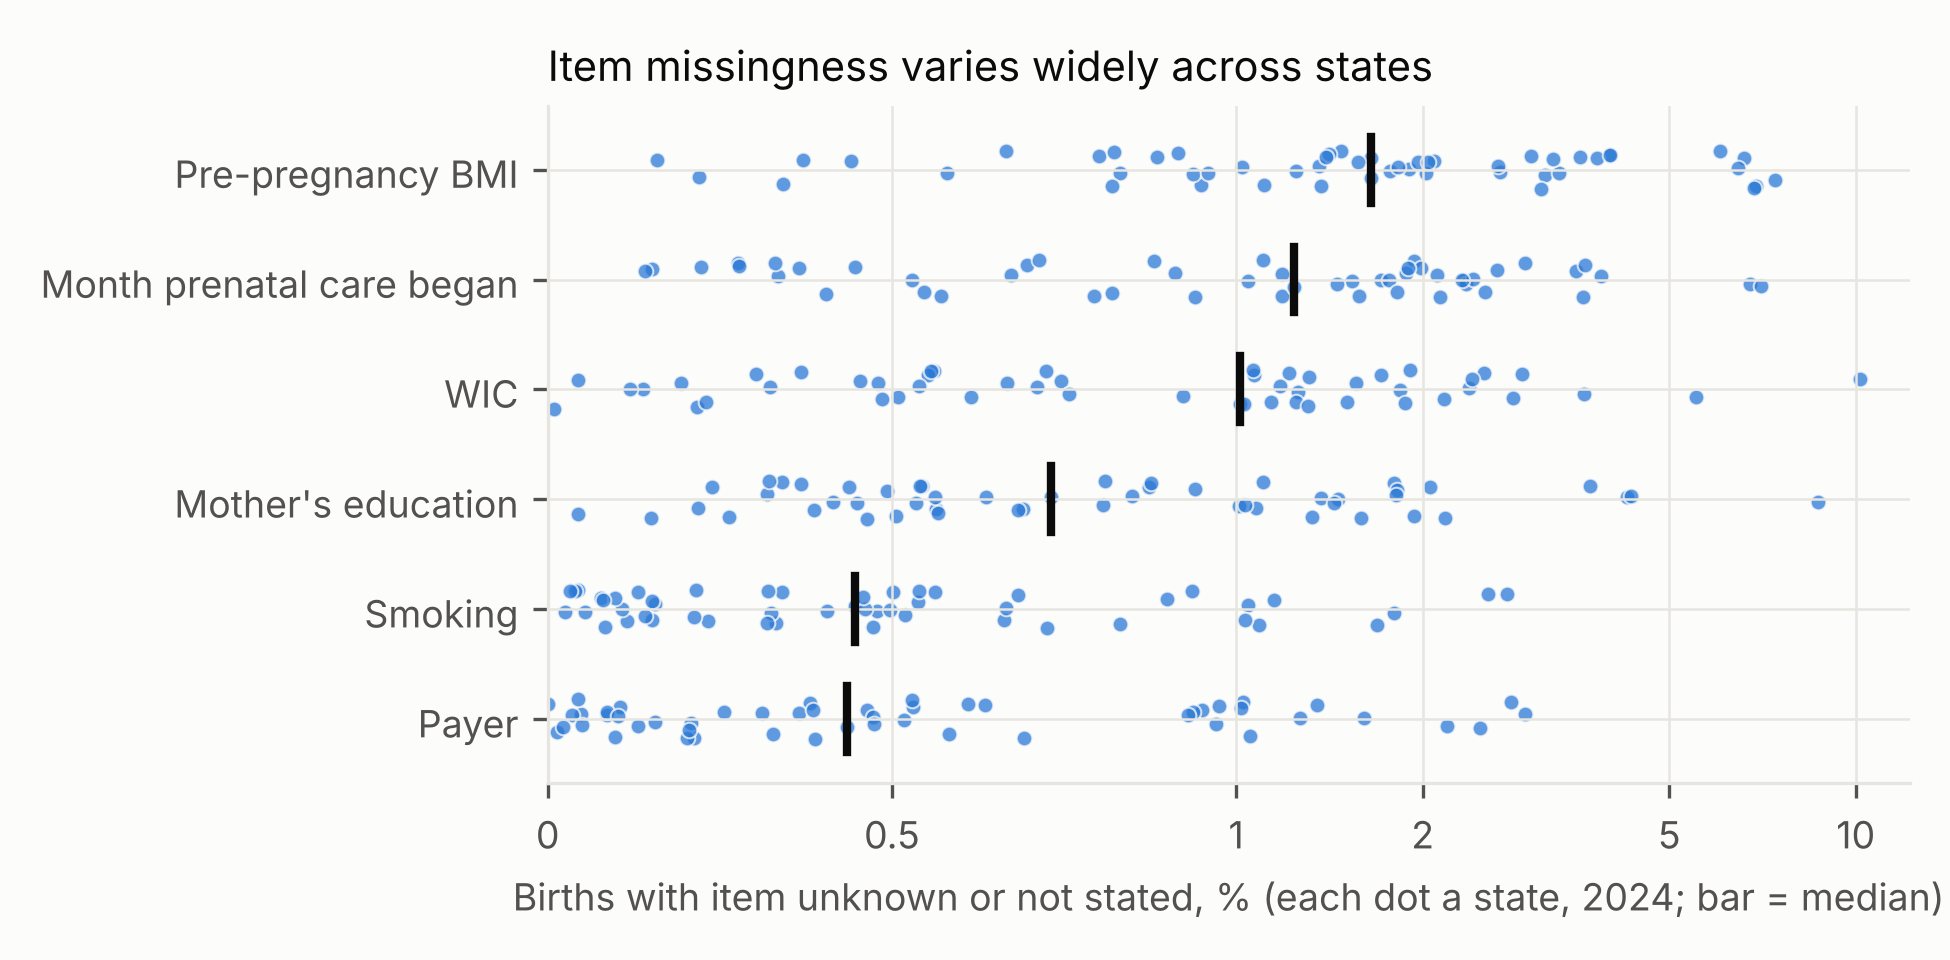
\includegraphics[width=0.85\textwidth]{figures/fig1_state_missingness.png}
\caption{Births with each item unknown or not stated, by state (\TestYear, CDC WONDER). Each dot is a state; bars mark the median state.}
\label{fig:missing}
\end{figure}

\paragraph{Simulated state missingness.} At observed rates every tree-based method stayed close to the full-information teacher (Table~\ref{tab:mar}, Figure~\ref{fig:gap}). For LBW the distilled students matched or slightly exceeded the teacher's PPV (median gap \LBWKDsPpvGap{} points for per-state students and \LBWKDpPpvGap{} for the pooled student); for PTB the teacher with mean imputation was closest (\PTBBonePpvGap{} points). Logistic regression with missing indicators had the lowest AUROC for both outcomes (\LBWBfourAuc{} for LBW and \PTBBfourAuc{} for PTB, against \LBWTAuc{} and \PTBTAuc{} for the teacher). Compared with the same learner trained on hard labels, the per-state distilled student had higher AUROC in \LBWKDhigherAuc{} of \NStudentsCompared{} states for LBW and \PTBKDhigherAuc{} of \NStudentsCompared{} for PTB, and higher PPV in \LBWKDhigherPpv{} and \PTBKDhigherPpv{} states, respectively. Calibration was slightly worse with distillation: the distilled student had the lower ICI in \LBWKDlowerIci{} of \NStudentsCompared{} states for LBW and \PTBKDlowerIci{} of \NStudentsCompared{} for PTB, although every ICI was below one percentage point (Figure~\ref{fig:ici}).

\begin{table}[H]
\centering
\small
\caption{Performance under state missingness simulated at observed rates (MAR masks), \TestYear{} births. Values are medians across all \NStates{} jurisdictions, except per-state models (medians across the \NStateStudents{} states with their own student). $\Delta$PPV and $\Delta$Sens.\ are differences from the full-information teacher in the same state, in percentage points, at the \AlertPct{} alert rate.}
\label{tab:mar}
\resizebox{\textwidth}{!}{\begin{tabular}{lrrrrrr}
\toprule
Model & AUROC & AUPRC (\%) & PPV (\%) & $\Delta$PPV & $\Delta$Sens. & ICI (\%)\\
\midrule
\multicolumn{7}{l}{\textit{Low birthweight}}\\
\quad Teacher, full information & 0.684 & 15.6 & 18.0 & -- & -- & 0.24\\
\quad Distilled student, per state & 0.683 & 15.5 & 18.1 & +0.10 & +0.09 & 0.23\\
\quad Distilled student, pooled & 0.683 & 15.5 & 18.2 & +0.11 & +0.08 & 0.26\\
\quad Non-distilled student, per state (B3) & 0.682 & 15.4 & 18.1 & +0.01 & $-$0.01 & 0.20\\
\quad Non-distilled student, pooled (B3) & 0.682 & 15.5 & 18.1 & +0.08 & +0.05 & 0.22\\
\quad Teacher + mean imputation (B1) & 0.683 & 15.5 & 18.0 & $-$0.03 & $-$0.01 & 0.24\\
\quad Teacher + iterative imputation (B2) & 0.682 & 15.2 & 17.9 & $-$0.09 & $-$0.15 & 0.25\\
\quad Logistic regression + indicators (B4) & 0.655 & 13.7 & 16.6 & $-$1.44 & $-$1.47 & 0.32\\
\addlinespace
\multicolumn{7}{l}{\textit{Preterm birth}}\\
\quad Teacher, full information & 0.672 & 19.1 & 22.8 & -- & -- & 0.46\\
\quad Distilled student, per state & 0.671 & 19.0 & 22.7 & $-$0.15 & $-$0.15 & 0.47\\
\quad Distilled student, pooled & 0.671 & 19.0 & 22.7 & $-$0.10 & $-$0.05 & 0.47\\
\quad Non-distilled student, per state (B3) & 0.669 & 18.8 & 22.7 & $-$0.19 & $-$0.13 & 0.44\\
\quad Non-distilled student, pooled (B3) & 0.670 & 18.8 & 22.6 & $-$0.26 & $-$0.14 & 0.42\\
\quad Teacher + mean imputation (B1) & 0.671 & 19.1 & 22.8 & $-$0.05 & $-$0.03 & 0.47\\
\quad Teacher + iterative imputation (B2) & 0.670 & 18.4 & 22.7 & $-$0.11 & $-$0.18 & 0.47\\
\quad Logistic regression + indicators (B4) & 0.644 & 17.4 & 21.4 & $-$1.44 & $-$1.70 & 0.60\\
\bottomrule
\end{tabular}
}
\end{table}

\begin{figure}[H]
\centering
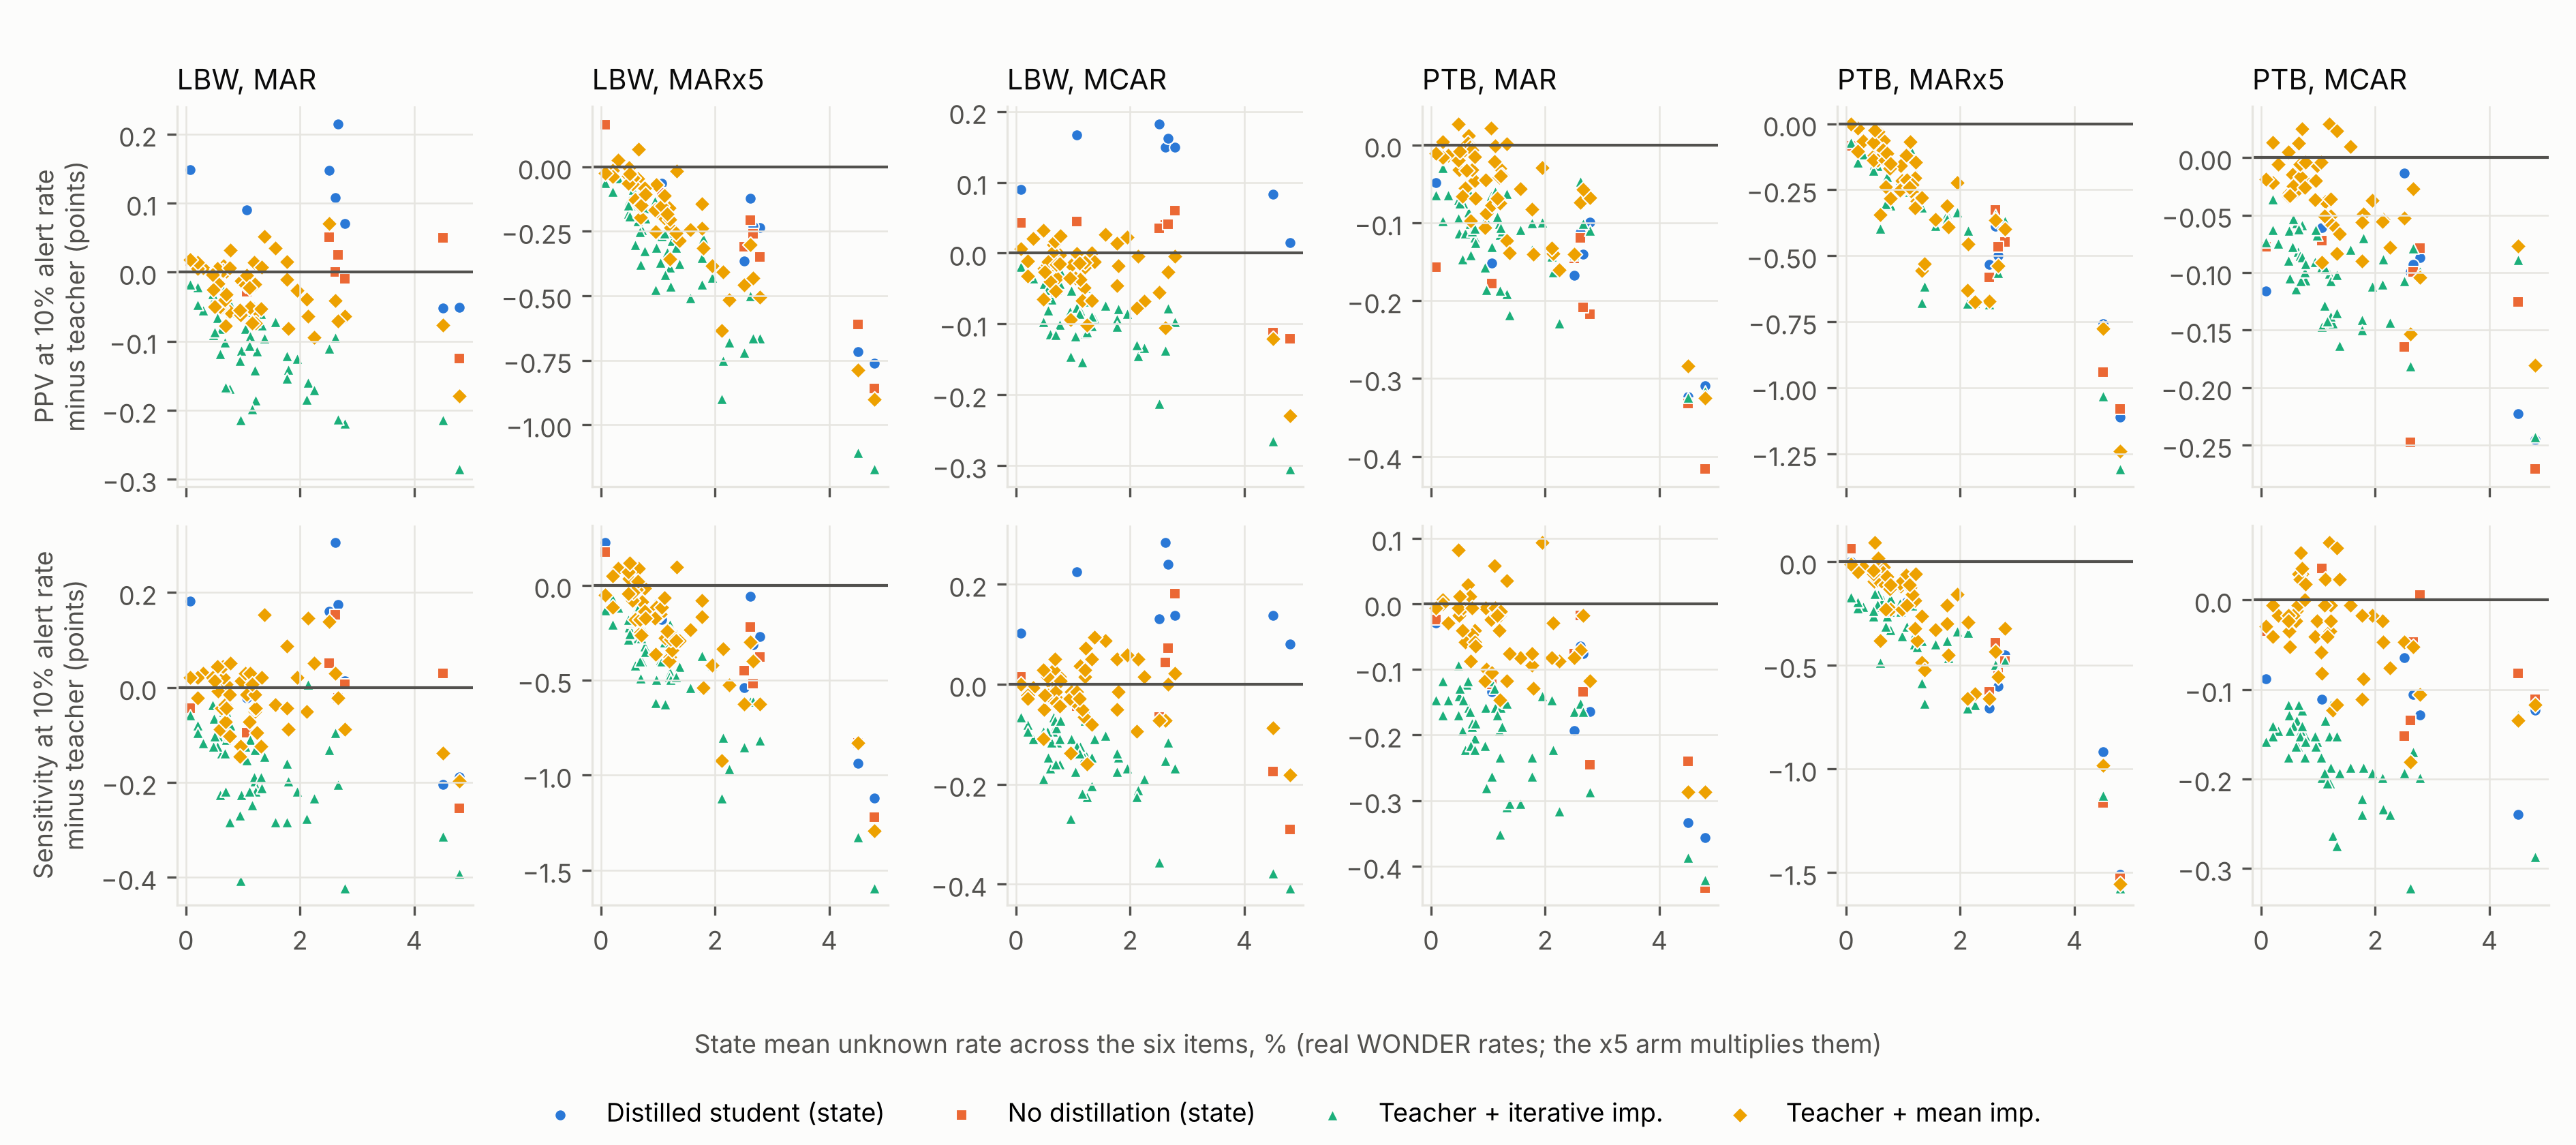
\includegraphics[width=\textwidth]{figures/fig2_gap_to_teacher.png}
\caption{Gap to the full-information teacher in PPV (top) and sensitivity (bottom) at the \AlertPct{} alert rate, by state, outcome and missingness mechanism.}
\label{fig:gap}
\end{figure}

\paragraph{Missingness mechanism.} Gaps were similar under MCAR and MAR masks (Table~\ref{tab:mech}). When every state's rates were multiplied by \StressMult, PPV relative to the teacher fell for every method, and the pooled students degraded least among the students.

\begin{table}[H]
\centering
\small
\caption{Median PPV gap to the full-information teacher (percentage points, \AlertPct{} alert rate) by missingness mechanism.}
\label{tab:mech}
\begin{tabular}{lrrr}
\toprule
Model & MCAR & MAR & MAR, rates $\times$5\\
\midrule
\multicolumn{4}{l}{\textit{Low birthweight}}\\
\quad Distilled student, per state & +0.15 & +0.10 & $-$0.23\\
\quad Distilled student, pooled & +0.17 & +0.11 & $-$0.04\\
\quad Non-distilled student, per state (B3) & +0.04 & +0.01 & $-$0.29\\
\quad Non-distilled student, pooled (B3) & +0.09 & +0.08 & $-$0.03\\
\quad Teacher + mean imputation (B1) & $-$0.02 & $-$0.03 & $-$0.16\\
\quad Teacher + iterative imputation (B2) & $-$0.08 & $-$0.09 & $-$0.29\\
\quad Logistic regression + indicators (B4) & $-$1.40 & $-$1.44 & $-$1.54\\
\addlinespace
\multicolumn{4}{l}{\textit{Preterm birth}}\\
\quad Distilled student, per state & $-$0.10 & $-$0.15 & $-$0.47\\
\quad Distilled student, pooled & $-$0.08 & $-$0.10 & $-$0.19\\
\quad Non-distilled student, per state (B3) & $-$0.11 & $-$0.19 & $-$0.46\\
\quad Non-distilled student, pooled (B3) & $-$0.14 & $-$0.26 & $-$0.24\\
\quad Teacher + mean imputation (B1) & $-$0.03 & $-$0.05 & $-$0.22\\
\quad Teacher + iterative imputation (B2) & $-$0.10 & $-$0.11 & $-$0.23\\
\quad Logistic regression + indicators (B4) & $-$1.40 & $-$1.44 & $-$1.54\\
\bottomrule
\end{tabular}

\end{table}

\begin{figure}[H]
\centering
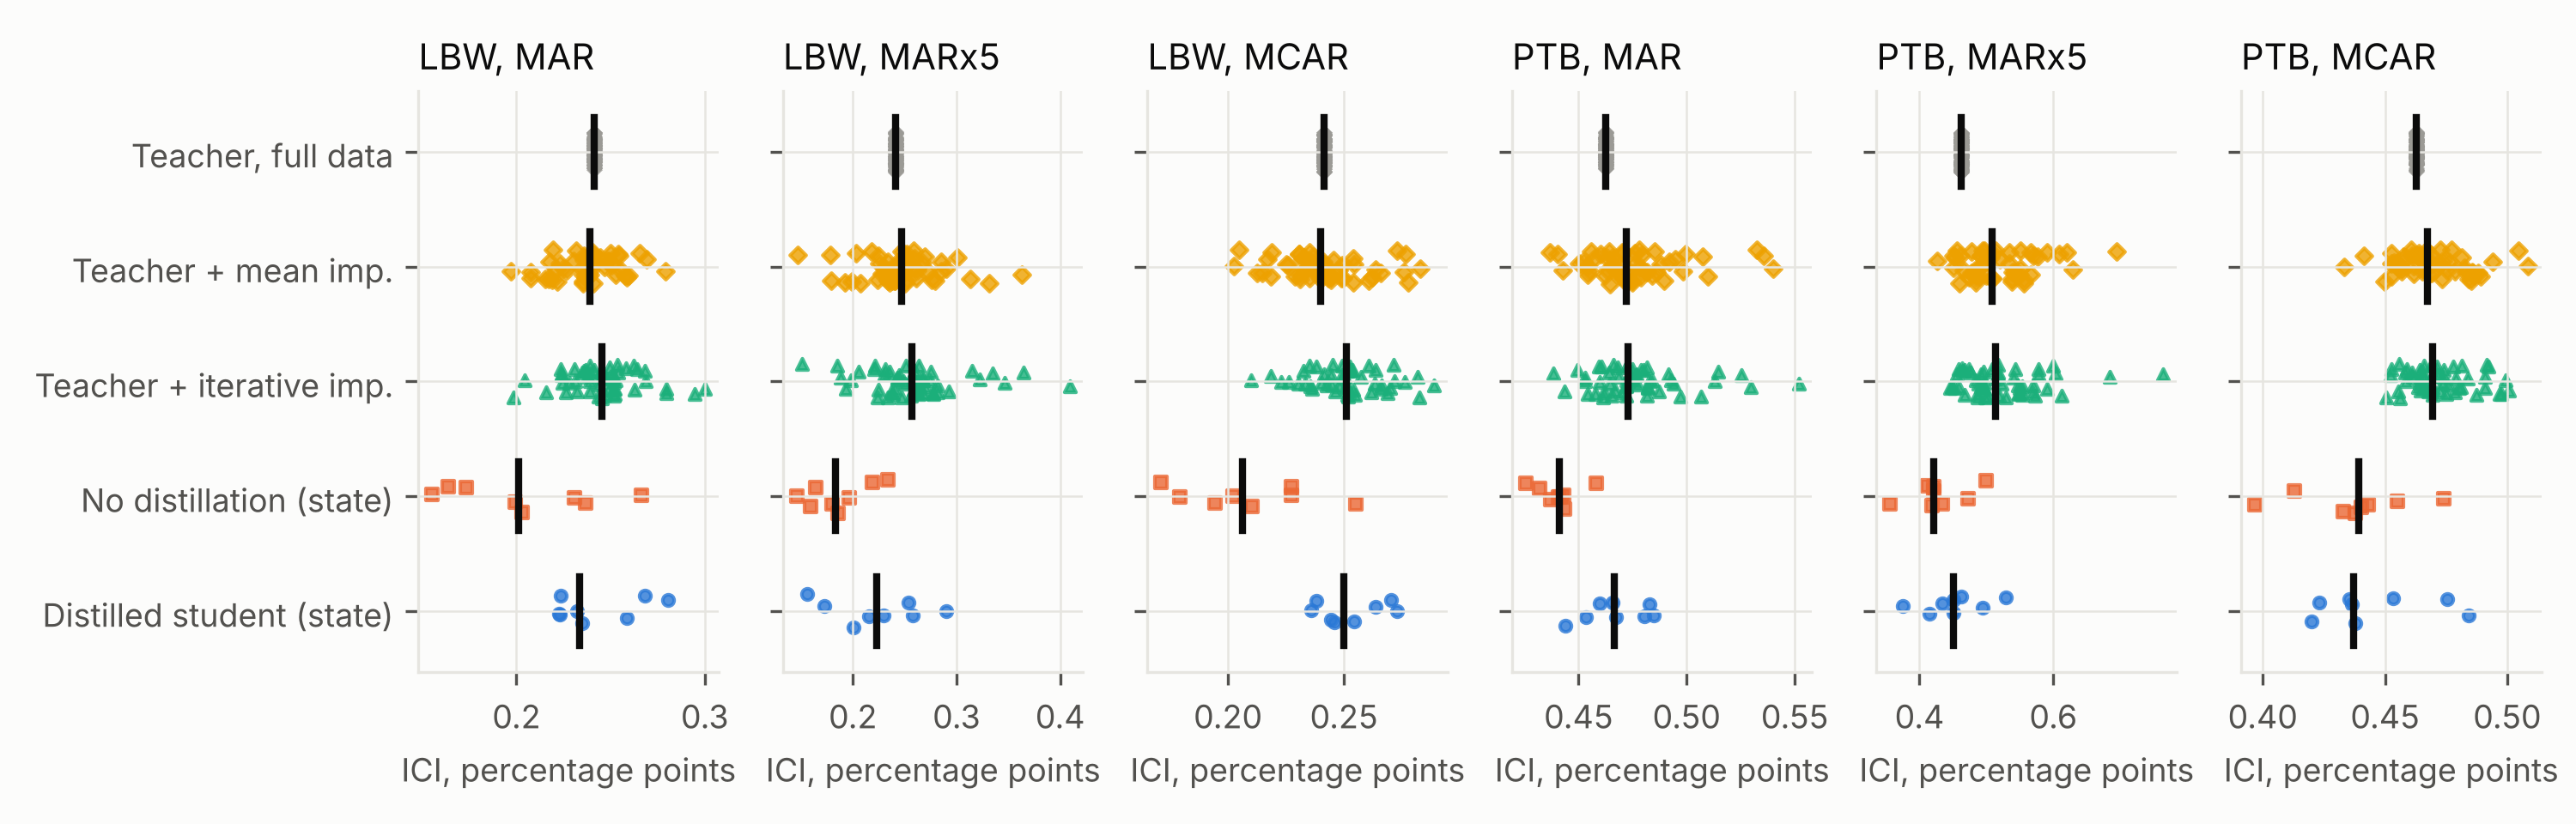
\includegraphics[width=0.9\textwidth]{figures/fig3_calibration_ici.png}
\caption{Integrated calibration index across states, by model, outcome and missingness mechanism.}
\label{fig:ici}
\end{figure}

\paragraph{Naturally missing items.} In \NaturalN{} test-year records with at least one item missing (\LBWNatEvents{} LBW and \PTBNatEvents{} PTB events), the pooled distilled student had the highest AUROC for both outcomes (\LBWNatKDAuc{} and \PTBNatKDAuc), and every paired interval for its AUROC advantage over mean imputation, iterative imputation and the non-distilled student excluded zero (Table~\ref{tab:natural}). The interval for its PPV advantage excluded zero over iterative imputation and over mean imputation for both outcomes, and over the non-distilled student for PTB but not LBW (LBW \LBWNatPpvThree{} points; PTB \PTBNatPpvThree).

\begin{table}[H]
\centering
\footnotesize
\setlength{\tabcolsep}{4pt}
\caption{Test-year records with at least one naturally missing item (models trained under MAR masks). PPV at the \AlertPct{} alert rate. The last two columns are paired bootstrap 95\% intervals for the pooled distilled student minus each comparator.}
\label{tab:natural}
\resizebox{\textwidth}{!}{\begin{tabular}{lllll}
\toprule
 & & & \multicolumn{2}{c}{Distilled minus comparator (95\% CI)}\\
\cmidrule(lr){4-5}
Model & AUROC (95\% CI) & PPV, \% (95\% CI) & AUROC & PPV (points)\\
\midrule
\multicolumn{5}{l}{\textit{Low birthweight}}\\
\quad Distilled student, pooled & 0.683 (0.679, 0.687) & 24.6 (24.2, 25.1) & -- & --\\
\quad Non-distilled student, pooled (B3) & 0.681 (0.677, 0.685) & 24.5 (23.9, 25.0) & +0.001, +0.003 & $-$0.05, +0.39\\
\quad Teacher + mean imputation (B1) & 0.677 (0.674, 0.682) & 24.3 (23.9, 24.9) & +0.004, +0.006 & +0.01, +0.61\\
\quad Teacher + iterative imputation (B2) & 0.669 (0.665, 0.673) & 23.4 (22.9, 23.9) & +0.013, +0.016 & +0.97, +1.61\\
\quad Logistic regression + indicators (B4) & 0.649 (0.645, 0.654) & 22.3 (21.9, 22.8) & +0.031, +0.036 & +1.95, +2.77\\
\addlinespace
\multicolumn{5}{l}{\textit{Preterm birth}}\\
\quad Distilled student, pooled & 0.685 (0.681, 0.689) & 31.6 (31.2, 32.2) & -- & --\\
\quad Non-distilled student, pooled (B3) & 0.682 (0.678, 0.686) & 31.4 (31.0, 32.0) & +0.002, +0.004 & +0.05, +0.43\\
\quad Teacher + mean imputation (B1) & 0.675 (0.671, 0.679) & 31.2 (30.7, 31.8) & +0.009, +0.011 & +0.24, +0.63\\
\quad Teacher + iterative imputation (B2) & 0.668 (0.664, 0.672) & 30.6 (30.2, 31.2) & +0.016, +0.018 & +0.75, +1.25\\
\quad Logistic regression + indicators (B4) & 0.647 (0.644, 0.651) & 29.2 (28.7, 29.9) & +0.036, +0.041 & +1.94, +2.82\\
\bottomrule
\end{tabular}
}
\end{table}

\paragraph{Subgroups.} PPV at the \AlertPct{} alert rate by maternal race and Hispanic origin, age band, payer and nativity is shown in Figure~\ref{fig:subgroups}. Among the tree-based methods, PPV differed by less than one percentage point in \SubTight{} of \SubCells{} outcome-by-subgroup cells, and no method was consistently best; logistic regression had the lowest PPV in \SubBfourLow{} of \SubCells. Larger differences occurred in smaller subgroups, where estimates are less precise.

\begin{figure}[H]
\centering
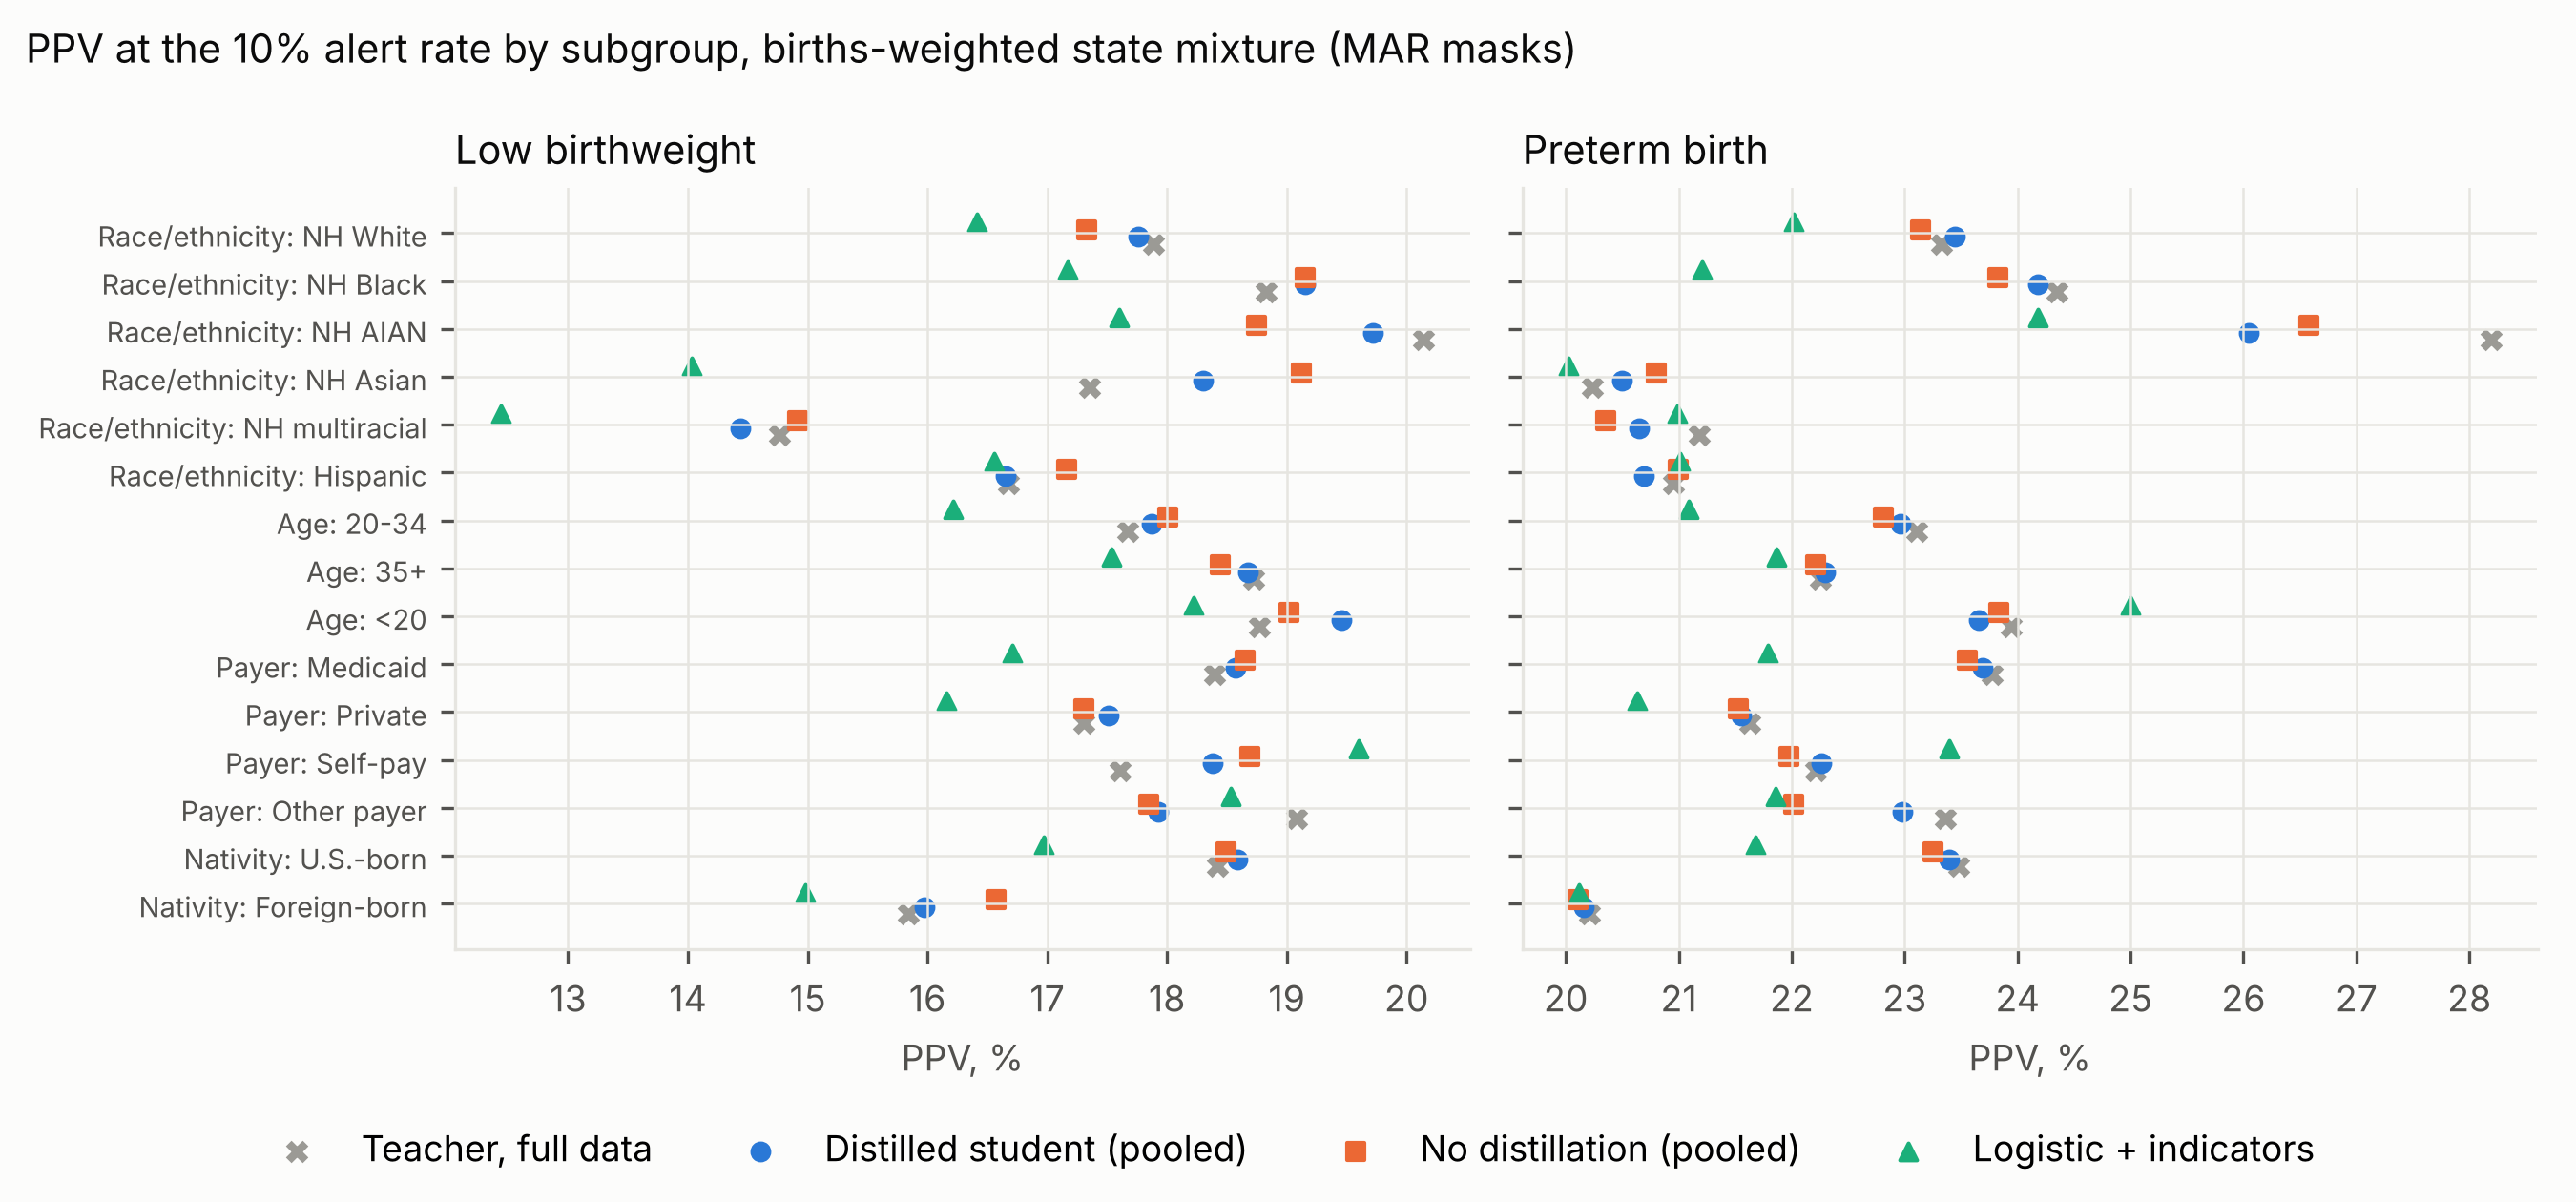
\includegraphics[width=0.9\textwidth]{figures/fig4_subgroups_ppv.png}
\caption{PPV at the \AlertPct{} alert rate by subgroup under the births-weighted state mixture (MAR masks).}
\label{fig:subgroups}
\end{figure}

\section{Discussion}\label{sec:discussion}

Two pictures emerge from these results. On simulated state missingness at the rates states actually report, every tree-based method stayed within a fraction of a percentage point of the full-information teacher's PPV, while logistic regression with missing indicators trailed by more than a point. Distilled students matched or slightly exceeded the teacher for low birthweight, whereas the teacher combined with simple mean imputation was as good or better for preterm birth. On real records with naturally missing items the ordering was clearer: the pooled distilled student had higher AUROC than every baseline for both outcomes, with bootstrap intervals that excluded zero, and higher PPV than both imputation approaches.

The two tests disagree for an identifiable reason. The simulated masks assume missingness that is completely at random or that depends only on observed covariates. Real unknown items on birth certificates are unlikely to behave that way: a blank prenatal-care field may itself reflect limited or late care, so missingness carries information about risk. Models trained on masked inputs with explicit missingness indicators can use that signal, whereas imputing a plausible value into a complete-data teacher discards it. This is consistent with arguments that missing-data handling for prediction should preserve, rather than remove, informative missingness \citep{sperrin2020,sisk2023}. Distillation added a small but consistent AUROC gain over the same learner trained on hard labels, in line with the view of soft targets as lower-variance supervision \citep{hinton2015,lopezpaz2016}, at the cost of slightly worse calibration.

Because real state-level item missingness is low, the practical benefit of any missing-data strategy for most jurisdictions is small. Where it matters most is in the records that are incomplete, which are not a random subset of births; there, a distilled student trained to expect missing items outperformed imputation. Per-state students did not improve on a single pooled student in this analysis, which suggests that one national student trained across state missingness patterns may be sufficient.

This study has limitations. State missingness was simulated from WONDER marginal rates because public-use files lack state identifiers, so the joint and outcome-related structure of real state missingness is not captured, and the natural-missingness analysis is national rather than state-specific. Training used \TrainYears{} only, because the 2018--2022 files were not available for this analysis. Predictors are recorded on the certificate at or after delivery, and completeness does not guarantee accuracy \citep{martin2013}. Only gradient-boosted trees were studied as teacher and student, own students were trained for \NStateStudents{} of \NStates{} jurisdictions, and subgroup results are descriptive.

\section{Conclusion}\label{sec:conclusion}

For low birthweight and preterm birth prediction from U.S.\ birth certificates, missingness-aware knowledge distillation performed comparably to imputation on simulated state missingness at real rates and better than imputation on records with naturally missing items. Evaluating models on naturally incomplete records, not only on simulated masks, changed the conclusion and should be standard practice when deployment-time missingness is at issue. Natural extensions are training on all available years, students for every jurisdiction, and validation in settings where state identifiers are available.

\section*{Use of AI tools}

Claude (Anthropic) was used to write and test analysis code, process data, search the literature, generate figures, and draft parts of the text. The author designed the study, made the modeling decisions, reviewed the manuscript, and takes responsibility for its content.

\section*{Data and code availability}

The NCHS natality public-use files and CDC WONDER are publicly available; no microdata are redistributed. Analysis code is available at \url{https://github.com/SelormB/makd-natality}.

\bibliographystyle{unsrtnat}
\bibliography{refs}

\end{document}
